\documentclass[a4paper,12pt,openright,twoside]{report}
\usepackage[british,UKenglish,USenglish,english,american]{babel}
%\usepackage[applemac]{inputenc}
\usepackage{newlfont}
\textwidth=450pt
\setcounter{secnumdepth}{3}
\oddsidemargin=10pt 
\evensidemargin=20pt 
\usepackage{graphicx}
\usepackage{indentfirst}
\usepackage{fancyhdr}
\usepackage{amssymb}
\usepackage{amsmath}
\usepackage{latexsym}
\usepackage{amsthm}
\usepackage{eucal}

\pagestyle{fancy}\addtolength{\headwidth}{20pt}
\renewcommand{\chaptermark}[1]{\markboth{\thechapter.\ #1}{}}
\renewcommand{\sectionmark}[1]{\markright{\thesection \ #1}{}}
\cfoot{}

\rhead[\fancyplain{}{\bfseries\leftmark}]{\fancyplain{}{\bfseries\thepage}}
\lhead[\fancyplain{}{\bfseries\thepage}]{\fancyplain{}{\bfseries\rightmark}}

\linespread{1.3}    
\theoremstyle{plain}                    
\newtheorem{theorem}{Theorem}[section]      
\theoremstyle{definition}               
\newtheorem{defin}{Definition}[chapter]

\begin{document}
%\documentclass[a4paper,12pt,openright,twoside]{report}
%\usepackage[british,UKenglish,USenglish,american]{babel}
%\usepackage{newlfont}
\textwidth=450pt\oddsidemargin=0pt

%\begin{document}
	\begin{titlepage}
		\begin{center}
			{{\Large{\textsc{Alma Mater Studiorum $\cdot$ Universit\`a di
							Bologna}}}} \rule[0.1cm]{15.8cm}{0.1mm}
			\rule[0.5cm]{15.8cm}{0.6mm}
			{\small{\bf SCUOLA DI SCIENZE\\
					Corso di Laurea in Informatica }}
		\end{center}
		\vspace{15mm}
		\begin{center}
			{\LARGE{\bf RANGE QUERIES ON AN}}\\
			\vspace{3mm}
			{\LARGE{\bf ENCRYPTED OUTSOURCED}}\\
			\vspace{3mm}
			{\LARGE{\bf DATABASE}}\\
			\vspace{3mm}
		\end{center}
		\vspace{40mm}
		\par
		\noindent
		\begin{minipage}[t]{0.47\textwidth}
			{\large{\bf Relatore:\\
					Prof. Ozalp Babaoglu}}\\
			{\large{\bf Co-relatore:\\
					Prof. Erkay Savas}}
		\end{minipage}
		\hfill
		\begin{minipage}[t]{0.47\textwidth}\raggedleft
			{\large{\bf Presentata da:\\
					Stefano Bernagozzi}}
		\end{minipage}
		\vspace{20mm}
		\begin{center}
			{\large{\bf III Sessione\\%inserire il numero della sessione in cui ci si laurea
					Anno Accademico 2014/2015 }}%inserire l'anno accademico a cui si è iscritti
		\end{center}
	\end{titlepage}
%\end{document}


\pagenumbering{roman}  
\chapter*{Abstract}

\addcontentsline{toc}{chapter}{Abstract}

A seguito della larga informatizzazione dei dati all'interno di tutti i settori, oggi la maggior parte dei nostri dati (sensibili e non) \`e memorizzata in qualche server in rete, del quale a volte non ne conosciamo n\`e ubicazione n\`e proprietario. 
Con lo sviluppo di questa tendenza, per\`o, \`e sempre pi\`u a rischio la sicurezza di tali dati, infatti sono sempre di pi\`u le notizie di attacchi informatici contro server per il recupero dei dati, ove poi viene fatto uso malizioso di essi. Tanto per citarne alcuni recenti sono famosi lo scandalo di dati rubati da Ashley Madison nel luglio 2015 \cite{madison} e il furto alla Sony nel dicembre 2014 \cite{sony}.\\
Per evitare che ci\`o accada si sta sempre pi\`u estendendo l'uso della crittografia, tramite la qual viene garantito all'utente l'uso esclusivo (o con un ristretto gruppo di persone) delle informazioni messe a disposizione dal server. 
Tale metodo per\`o non \`e sufficiente a garantire la confidenzialità di tali dati in quanto nella maggior parte di casi i dati sul server sono in chiaro e se volesse il proprietario del server potrebbe recuperare tali dati e venderli o mostrarli in pubblico. Inoltre tramite questo metodo se un criminale informatico riuscisse a ottenere l'accesso al server, potrebbe tranquillamente recuperare i dati senza che nessuno lo scopra. 
Proprio per questo il metodo migliore \`e crittografare i dati sul server, di modo che anche chi ha accesso a tali dati non li pu\`o recuperare a meno che non possegga la chiave per decifrarli.\\
Di seguito analizzeremo un metodo per realizzare tale sicurezza e anche il modo in cui implementarlo successivamente su di un elaboratore.\\
Il metodo analizzato in questo documento riguarda l'utilizzo della struttura b+tree per l'archiviazione di dati crittografati, in particolare viene utilizzato dal client per ricreare l'indice di un database su una chiave anche non primaria per poi effettuare una ricerca su tale indice.
I dati per\`o, che inizialmente sono salvati su di un file o inseriti manualmente dall'utente, vengono successivamente criptati e spediti al server, di modo che esso non possa recuperare i dati al suo interno. Successivamente a seguito dell'esecuzione di una query da parte del cliente sul database, i dati vengono recuperati a partire dalla radice dell'albero e vengono tenuti in cache per effettuare le query pi\`u velocemente. Quando il client ha terminato di utilizzare il database tutti i nodi dell'albero in memoria vengono scambiati di settore e rispediti al server, crittografandoli anche con un salting diverso. Inoltre per garantire che il server non intuisca quali settori vengono recuperati, vengono effettuate delle "fake searches", cio\`e al momento di recuperare ogni nodo si guardano i figli e se ne ha piu' di uno vengono recuperati alcuni settori che possono non essere utili.


\tableofcontents{}

\clearpage{\pagestyle{empty}\cleardoublepage}
\chapter{Introduction}
\pagenumbering{arabic}
\section{Problem formalisation}
This project is about retrieving data in range without allowing the server to read it, and also to relate the queries and the nodes in memory. 
Basically, our goal is to build a database that allows the client to maintain the confidentiality of the data stored, despite all the data is stored in a different location from the client's hard disk. This means that all the data written on the hard disk can be easily read by another person who can do anything with it. 
Given that, we need to encrypt that data from eavesdroppers or other people. This is because they could sell it or login into accounts and use them for stealing money or identities. In order to achieve this, we need to encrypt the data stored in the hard drive, so that only the one who has the key can easily read the information stored, while all the others are going to read only encrypted data.
Obviously, according to that, all the data management must be done by the client, otherwise any malicious person can easily retrieve it and use it for any malicious intention.
The first chapter concerns about introducing the structures used for the realization of the project and some technical terms necessary for the second part.
\\
The second chapter examines various encrypted databases, and explain the methods that they use for realize such purpose.
\\
The third chapter concerns about the implementation of the project and its details.
\\In the fourth chapter there is the testing of the project over some databases.
\\Concluding the last chapter explain the results obtained and the future work based on this project, with some possible uses of it.

%(the server retrieve what? And the server use it for bad purposes? This last sentence needs to be reviewed. Apart from this, now the English is quite good. You should explain more than "why we need to encrypt the data" how you retrieve data in range, since as I understood it's the main part of the thesis!

\section{Background knowledge}
\subsection{B+tree}
A B+tree is a data structure used for ordering the keys in a database. Each node has a large number of children. They are used in many contexts, from filesystems, like NTFS, to databases. It is indexed on a single key and, differently from a standard binary tree, all the data is stored under the leaves, as it is shown in figure 1. This means that, if we want to retrieve a record from this database, we have a complexity of $o(h)$ where $h$ is the height of the tree. 
The root and the internal node have more than $\frac{n}{2}$ children, where $n$ is the maximum number of children that a node can have. All the data under the leaves is linked by a pointer that points to the record. %with that key
%In each internal node, all the keys %that between the searched key is located between the nearest pointers (one lower and one higher). 
Searching the specified key on this data structure can be easily made by following the path denoted by the keys in the internal nodes. It has a complexity of $O(\log{} _a n)$, where a is the branching factor of the tree and n is the height of the tree (defined as the number of levels in the tree).
In our implementation we don't have any link between the leaves, that means we have to start from the parent for retrieve any sibling of the node, and also we have to start from the root to do range queries. We used this implementation because in order to to preserve the tree we need to keep in memory all the nodes between the root and the current, so that each node we retrieve, including the ones recovered from fake searches, must be attainable from the root.
  %not only that for retrieve every leaf we must begin from the parent but also a different approach for do a range query.
\\

\begin{figure}[htbp]
\centering
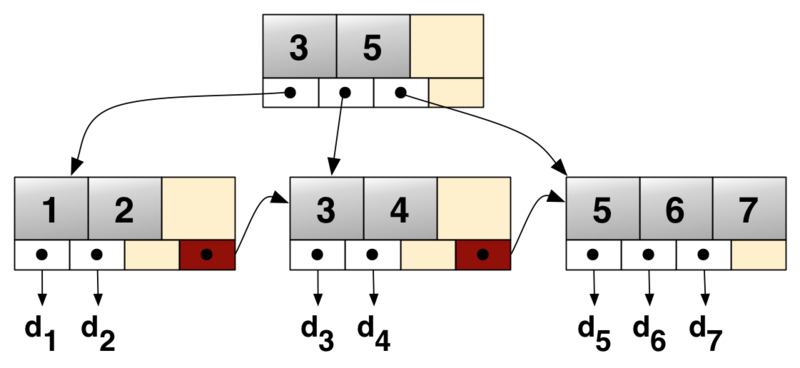
\includegraphics[scale=0.8]{bplustree.png}
\\Figure 1: A graphical representation of a b+tree (source www.wikipedia.org)
\end{figure}
\newpage
\subsection{AES algorithm}
The AES algorithm (also called Rijndael from its creators Vincent Rijmen and Joan Daemon), is a symmetric encryption algorithm. Symmetric means that the same key is used both for encrypting and decrypting. It became effective in 2002, after the approval of NIST. This algorithm is a block chiper, i.e. it processes blocks of fixed length (128 bit) arranged on a matrix (called \textbf{State Array}) where the first word (each word is four bytes) is in the first column and so on. 
$State Array = 
\begin{bmatrix}
s_{0,0} & s_{0,1} & s_{0,2} & s_{0,3} \\ 
s_{1,0} & s_{1,1} & s_{1,2} & s_{1,3} \\
s_{2,0} & s_{2,1} & s_{2,2} & s_{2,3} \\
s_{3,0} & s_{3,1} & s_{3,2} & s_{3,3} \\
\end{bmatrix}
$
The algorithm is composed of k rounds (as it is shown in figure 2) where k  depends on the key length. In our case we have a 128 bit key, that means AES standard, therefore we have k equal to 10 plus the first add round key  (in case of 196 bits k is 12 and 14 in case of 256 bits key).
\newpage
\begin{figure}[htbp]
\centering
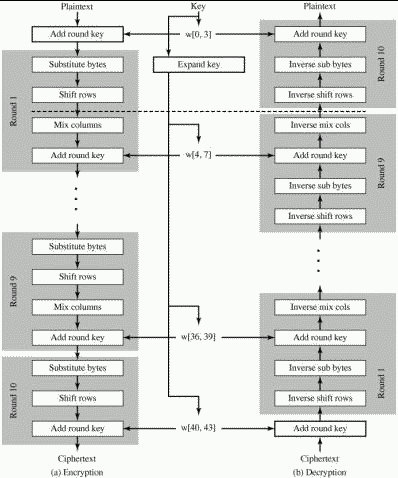
\includegraphics[scale=1]{AES_structure.png}
\\Figure 2: AES structure (source http://www.codeproject.com)
\end{figure}

\subsection{Key expansion algorithm}

Before applying the algorithm the key must be expanded, because at each step the add round key needs a portion of it. It is designed to ensure that a minimum change in the key (just only one bit is enough) should affect the next round keys for several times. A 128 bit key is expanded in the following manner: 
First is divided in 4 words as below:
\newpage

\begin{center}
$\begin{bmatrix}
k_0 & k_1 & k_2 & k_3\\
k_4 & k_5 & k_6 & k_7\\
k_8 & k_9 & k_10 & k_11\\
k_12 & k_13 & k_14 & k_15\\
\end{bmatrix}$\\
$\Downarrow$\\
$
\begin{bmatrix}
w_0 & w_1 & w_2 & w_3
\end{bmatrix}$\\
\end{center}
After this step the algorithm proceed four word at a time, as it is shown below in figure 4.\\
\begin{figure}[htbp]
	\centering
	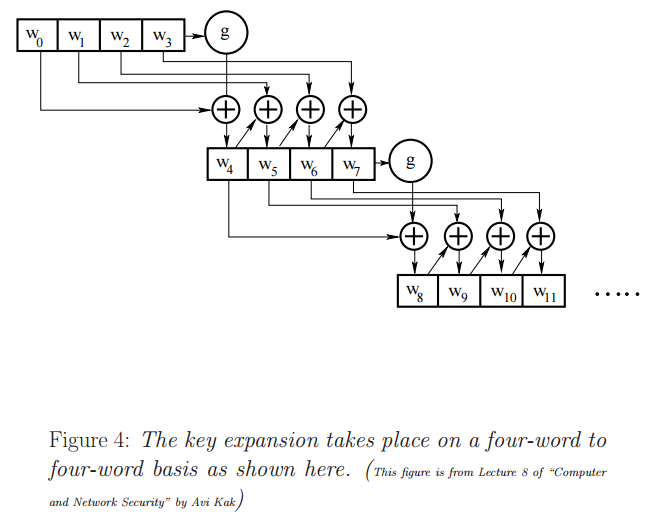
\includegraphics[scale=0.7]{key_expansion.png}
\end{figure}
\\Where $\oplus$ is the addition modulus 2 between the bits of the words and $g$ is a mathematical function as below.
$g()$ is composed by 3 steps: 
\begin{enumerate}
	\item One-byte left circular rotation on the 4 byte word.
	\item Byte substitution for each byte of the word returned using the lookup table taken from the Substitute Bytes step.
	\item XOR the bytes obtained from the previous step with a round constant. This step is important to destroy any symmetry that can exists in the previous steps.\\
	The round constant is derived at each round with the following formula (i starting from 1 is the number of the round):\\
	$Rcon[i] = (RC[i], 0x00, 0x00, 0x00)$\\
	Where:\\
	$RC[1] = 0x01$\\
	$RC[j] = 0x02 \times RC[j-1]$
\end{enumerate}


\subsubsection{Encryption}
Each round, except for the first (that is only an add round key) and the last, is composed by 4 steps:
\begin{enumerate}
\item substitute bytes
\item shift rows
\item mix columns
\item add round key
\end{enumerate}

The last round doesn't have the mix columns step in order to make the algorithm reversible. 
\paragraph{Substitute Bytes: }
The bytes substitution in the encryption works by replacing each byte with the corresponding value in the S-BOX, that is a $16\times16$ matrix (as it is shown below in figure 3). The lookup table is shown in hexadecimal value.
\newpage
\begin{figure}[htbp]
\centering
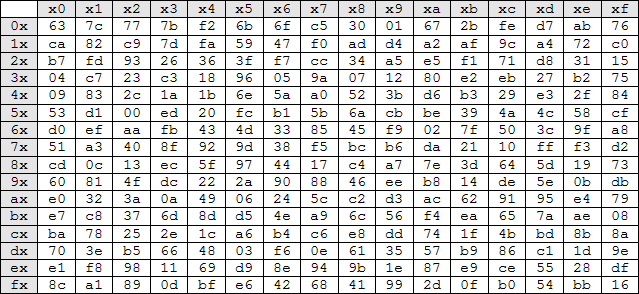
\includegraphics[scale=0.7]{sbox.png}
\\Figure 3: S-BOX (source https://edipermadi.wordpress.com)
\end{figure}
In this step the lookup table cannot be described as a mathematical function so the algorithm has to access the table every time.\\


\paragraph{Shift Rows: }
During the shift rows step each row of the state array is shifted as following:\\
\begin{center}
$
\begin{bmatrix}
s_{0,0} & s_{0,1} & s_{0,2} & s_{0,3} \\ 
s_{1,0} & s_{1,1} & s_{1,2} & s_{1,3} \\
s_{2,0} & s_{2,1} & s_{2,2} & s_{2,3} \\
s_{3,0} & s_{3,1} & s_{3,2} & s_{3,3} \\
\end{bmatrix}
\implies
\begin{bmatrix}
s_{0,0} & s_{0,1} & s_{0,2} & s_{0,3} \\ 
s_{1,1} & s_{1,2} & s_{1,3} & s_{1,0}\\
s_{2,2} & s_{2,3} & s_{2,0} & s_{2,1} \\
s_{3,3} & s_{3,0} & s_{3,1} & s_{3,2} \\
\end{bmatrix}
$
\end{center}
\paragraph{Mix Columns}
The mix columns step is composed by four operations, one for each row of the state array, as it is shown below:

\begin{itemize}
	\item For the first row the operation can be stated as: 
	$s'_{0,j} = (0x02 \times s_{0,j}) \otimes (0x03 \times s_{1,j}) \otimes s_{2,j} \otimes s_{3,j})$
	\item For the second row the operation can be stated as: 
	$s'_{1,j} = s_{0,j} \otimes (0x02 \times s_{1,j}) \otimes (0x03 \times s_{2,j}) \otimes s_{3,j})$
	\item For the third row the operation can be stated as: 
	$s'_{2,j} = s_{0,j} \otimes s_{1,j} \otimes (0x02 \times s_{2,j}) \otimes (0x03 \times s_{3,j}))$
	\item For the fourth row the operation can be stated as: 
	$s'_{3,j} = (0x03 \times s_{0,j}) \otimes s_{1,j} \otimes s_{2,j} \otimes (0x02 \times s_{3,j}))$
\end{itemize}

Or more compactly:
$
\begin{bmatrix}
02 & 03 & 01 & 01 \\ 
01 & 02 & 03 & 01 \\
01 & 01 & 02 & 03 \\
03 & 01 & 01 & 02 \\
\end{bmatrix}
\times
\begin{bmatrix}
s_{0,0} & s_{0,1} & s_{0,2} & s_{0,3} \\ 
s_{1,0} & s_{1,1} & s_{1,2} & s_{1,3} \\
s_{2,0} & s_{2,1} & s_{2,2} & s_{2,3} \\
s_{3,0} & s_{3,1} & s_{3,2} & s_{3,3} \\
\end{bmatrix}
=
\begin{bmatrix}
s'_{0,0} & s'_{0,1} & s'_{0,2} & s'_{0,3} \\ 
s'_{1,0} & s'_{1,1} & s'_{1,2} & s'_{1,3} \\
s'_{2,0} & s'_{2,1} & s'_{2,2} & s'_{2,3} \\
s'_{3,0} & s'_{3,1} & s'_{3,2} & s'_{3,3} \\
\end{bmatrix}
$

\paragraph{Add round key}

The add round key step is done by XORing each byte of the state with the relative byte of the key expanded. In the first round the input block is XORed with the first 4 words of the expanded key, and then at each of the following rounds the block is XORed with the next 4 words at a time.

\subsubsection{Decryption}
Each round, as it works in the encryption, is composed by 4 steps (first add round key and last round excluded):
\begin{enumerate}
\item substitute bytes
\item shift rows
\item mix columns
\item add round key
\end{enumerate}
\paragraph{Inverse Substitute Bytes: }
Like in the encryption, the bytes substitution is made by replacing every byte with the corresponding value. Differently from the encryption the value is searched in the inverse S-BOX (as it is shown below in figure 4).

\begin{figure}[htbp]
\centering
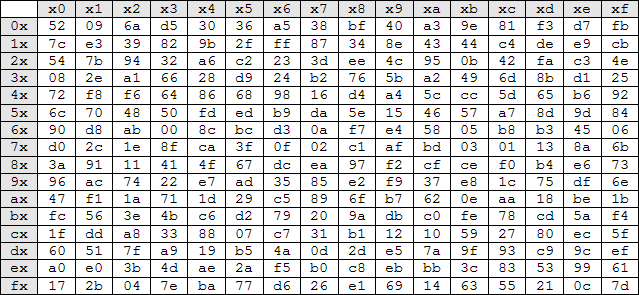
\includegraphics[scale=0.7]{isbox.png}
\\Figure 4: Inverse S-BOX (source https://edipermadi.wordpress.com)
\end{figure}

\paragraph{Shift rows}
During the shift rows step each row of the state array is shifted as following:\\
\begin{center}
	$
	\begin{bmatrix}
	s_{0,0} & s_{0,1} & s_{0,2} & s_{0,3} \\ 
	s_{1,0} & s_{1,1} & s_{1,2} & s_{1,3} \\
	s_{2,0} & s_{2,1} & s_{2,2} & s_{2,3} \\
	s_{3,0} & s_{3,1} & s_{3,2} & s_{3,3} \\
	\end{bmatrix}
	\implies
	\begin{bmatrix}
	s_{0,0} & s_{0,1} & s_{0,2} & s_{0,3} \\ 
	s_{1,3} & s_{1,0} & s_{1,1} & s_{1,2}\\
	s_{2,2} & s_{2,3} & s_{2,0} & s_{2,1} \\
	s_{3,1} & s_{3,2} & s_{3,3} & s_{3,0} \\
	\end{bmatrix}
	$
\end{center}
\paragraph{Mix columns}


The mix columns step is composed by four operations, one for each row of the state array, as it is shown below:

$
\begin{bmatrix}
0E & 0B & 0D & 09 \\ 
09 & 0E & 0B & 0D \\
0D & 09 & 0E & 0B \\
0B & 0D & 09 & 0E \\
\end{bmatrix}
\times
\begin{bmatrix}
s_{0,0} & s_{0,1} & s_{0,2} & s_{0,3} \\ 
s_{1,0} & s_{1,1} & s_{1,2} & s_{1,3} \\
s_{2,0} & s_{2,1} & s_{2,2} & s_{2,3} \\
s_{3,0} & s_{3,1} & s_{3,2} & s_{3,3} \\
\end{bmatrix}
=
\begin{bmatrix}
s'_{0,0} & s'_{0,1} & s'_{0,2} & s'_{0,3} \\ 
s'_{1,0} & s'_{1,1} & s'_{1,2} & s'_{1,3} \\
s'_{2,0} & s'_{2,1} & s'_{2,2} & s'_{2,3} \\
s'_{3,0} & s'_{3,1} & s'_{3,2} & s'_{3,3} \\
\end{bmatrix}
$

\paragraph{Add round key}
The add round key step in the decryption is the same as the encryption.


         

\clearpage{\pagestyle{empty}\cleardoublepage}
\chapter{State of the art}
At the date of writing, there are several implementations of encrypted databases.
Since the server is a part that cannot be fully trusted, most of the implementations are supposed to encrypt the data before it reaches the server. 
There are many levels of encryption, depending on how the data is encrypted and if it is all encrypted or only a part of it.
Another important aspect is how data is managed: in many cases data is only stored encrypted while all the process is done in cleartext, meanwhile some databases have implemented various algorithms for processing data in their encrypted form, so they don't have to manage cleartext.
According to these various methods we can divide them into 3 main categories:
\section{Data encryption at rest}
This type of encryption is also called TDE (Transparent Data Encryption) because is transparent to the user. 
The algorithm works by encrypting the database after the client ends the connection, and stores it to the disk ciphered, to prevent any malicious attacker from reading the database while it is not used. Of course, unless they recover the key. After that, it restores the database in plaintext only when the client needs to update it, so only in that moment the attacker can read it. A graphical representation of the algorithm is shown in figure 5. 
Encrypting data at rest has the advantage that one doesn't have to change the application level. In particular, all the applications that execute queries over the database remain the same. 
This means that all the data is in cleartext while the computation is done and, most important thing, while it is being sent through the network. This implies that any malicious eavesdropper can read any query or data retrieved and use it for his purposes.  
The first TDE implementation was done by Microsoft in SQL Server 2008 \cite{microsoft}.
Following Bill Gates's company, IBM \cite{ibm} and Oracle \cite{oracle} have implemented their own encrypted databases of this type. 
The company with headquarters in New York has implemented a software co-related with DB2, while Oracle has upgraded his own database.
Due to the passage of cleartext over the network this implementation is not related to our work, despite this type of database is widely used, since is the most transparent and quick encryption for a database. 
The interesting thing about this type of encryption is that can be integrated to record/column encryption, so it can add more security to the database (but increases the query time because of the double encryption). An implementation like the last one was done by Google\cite{google}.
Such algorithm can also be used for encrypting filesystems, like has done Windows with EFS\cite{efs}.\\
\begin{figure}[]
	\centering
	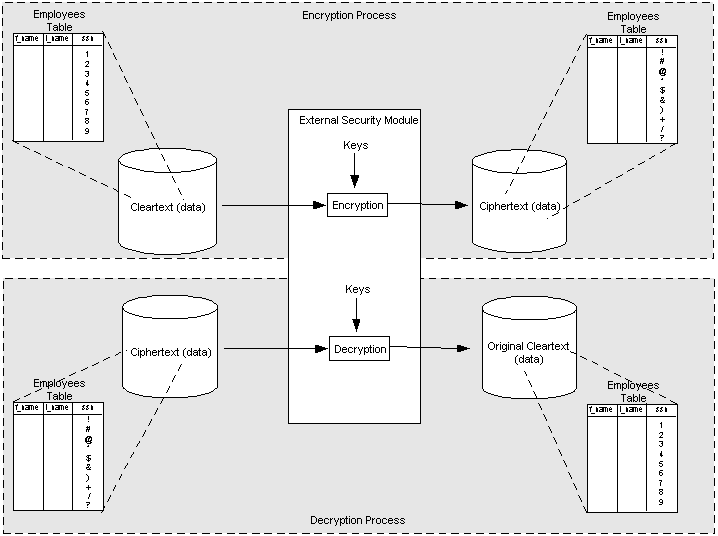
\includegraphics[scale=0.55]{transdata.png}
	\\Figure 1: A graphical representation Transparent Data Encryption (source www.oracle.com)
\end{figure}
\newpage


\section{Data encryption in transit}
The second method for encrypting data is to encrypt them "in transit", that means all the computation is done in plaintext. The advantage is that since the computation occurs client side, the data is encrypted before it is sent to the server, so all the packages that go through the network are ciphered, so if an eavesdropper recovers them, they cannot use them for malicious purposes.
This implementation relies on ciphering the single column of the database or, as it is in our case, single cells/records of it.
This method is widely used for filesystems, but today many companies are implementing it in their databases, since this ensure the client more security.
With data encryption in transit we have a reduction of the computation in the server.
The algorithm however must not be confused with public key cryptography, because with the last one the server has to decrypt the data. 
This method has been studied in the USA by \cite{cina}.


\section{Data encryption in use}
The last method relies on manage encrypted data, this means as soon as the data is inserted by the user it is encrypted in a particular manner. This allows the server to retrieve the data although it is encrypted. The implementation of this databases relies on homomorphic encryption, which is a type of encryption that allows manipulation over encrypted data\cite{homo1}\cite{homo2}. It has been studied in various articles, like \cite{tamper} and \cite{hard}.

\section{Our Approach}
Our approach is based on the data encryption in transit. In fact we encrypt all the packets before sending them to the server. The only information that the server have in plaintext are: the length of the data received and the initialization vector. Since this last is different for each encryption it must be added to the data. Other information that the server can retrieve are the level of the sector in the tree, but cannot reconstruct it. 

\clearpage{\pagestyle{empty}\cleardoublepage}
\chapter{Implementation}
Our implementation is based on C++ programming language. Most of the computation is done by the client, since the server cannot know which data is manipulating. This method allows the client to maintain the control over the cleartext data. In particular, the server cannot read it unless it recovers the key from the client. This maintains very strong the security of the database, since no one that has access to the server can obtain the true information from the data.

\section{Server}
The server side is very small in this program because of the confidentiality of the data. Due to this, the only task of the server is to interact between the client and the hard disk.
Is implemented in C++ but most of its parts are written in C. \\
When the server is launched it binds to a port, that is the argument passed by the client. in case of error it exits. After that it starts listening over the socket for some data. This part has 2 functions, that are \emph{readn} and \emph{writen}, which respectively read and write n bytes from and to the socket. They are made to process exactly n bytes, so the function doesn't end until they are all read/written.\\
During the listening, the server waits for a connection. When the server receives the attempt of a connection from a client, it launches a thread and accepts the connection. After that, it waits for a command. The accepted commands are the followings:
\begin{itemize}
\item "\textbf{wr}" which means that the client wants to write some data. The server waits for the sector where the client wants to write the data and the length of the data. In this case the server waits for the number of the sector and converts it from network integer representation to the host one. 
The same thing is done with the size of the data to write (the server always receives 512 Bytes). After that, it allocates an array of char where to store the data sent by the client. Done this, it receives the data from the client, that is the most important thing. 
When all the data is retrieved, the thread handling the client connection gets the mutual exclusion, and writes it into the disk.
This last part is done by seeking the hard drive sector with lseek and writing into it with the write function from the C library.
If there are no errors, the thread release the mutual exclusion, re-sends the number of the sector to the client for acknowledgment and frees the array previously allocated.
\item "\textbf{re}" means that the client wants to read a sector. The server waits for the sector's number, then, as it occurs for the previous command, command it converts the integer from network to host byte representation. Afterwards, the thread takes the mutual exclusion and reads the specified sector, by seeking it with lseek and reading it with the read function from C. In this case we don't need to receive the length of the data because the server automatically reads all the sector.
This string is put into a buffer previously allocated and then it is sent  to the client. Finally, the thread releases the mutual exclusion and frees the buffer.
\item "\textbf{xx}" which means that the client wants to close the connection. In such case, the server replies with "xx" message and then closes the socket.

\end{itemize}
The server is supposed to run in another computer instead of the client's one, and its workload is very small. Therefore, the client's computer doesn't have to be a powerful one. Due to this, the server can also be on the same computer of the client, even though the client has usually a not so powerful computer.

\section{Client}
Since most of the computation is done by the client, this part is the most important of the project. This section is divided into ... parts: the first one is related to the implementation of the b+tree and how to serialize it, the second part is related on how to encrypt all the sections of the tree and the third one is related on how and when interact with the server for retrieve the data.
Obviously if the server has no data stored, the client begins locally a new tree and after it has create all the tree with local data, it can do search operations on them and after that it sends all the data to the server for storing it.
For the cryptography is used the openssl library, that implements an AES 256 bit. For more information see \cite{openssl}. 
\subsection{B+tree implementation}
The code is based on a b+tree written in C (for more specification see \cite{bplustree}) with some changes: our implementation has no link between the leafs, is encrypted and stores the nodes in an external hard drive.
The structures used for the realization of the tree are:
\begin{itemize}
    \item \emph{node:} A node is the internal part of the tree and is composed by:
    \begin{itemize}
        \item a key that is a 32 bit integer;
        \item an array of keys, that associated with the pointers array and the sectors array 
        \item an array of sectors;
        \item an array of pointers;
        \item a pointer to the parent node;
        \item an integer that counts the number of the keys;
        \item an integer that mantain the sector in which it was stored.
    \end{itemize}
    it is important to distinguish between leafs and internal nodes because in the leafs the pointers corresponds to the pointers of the record with that key, while in the internal nodes the first pointer points to a node that contains the keys lower than the first key, the second points to a node with keys higher or equal to the first key and lower than the second and so on until the last node that points to a node with keys higher or equal to the last-1 key.
    \item \emph{record:} A record is the part of the tree where all the data is stored. It is collocated on the leafs of the tree and is composed by:
    \begin{itemize}
        \item a 32 bit integer that is the key;
        \item a pointer to an array of fields, in which are stored all the fields of the database. It isn't allocated before for allowing the client to choose the number of fields.
        \item a pointer to the parent node
        \item an integer that is the number of the sector.
    \end{itemize}
    \item \emph{info:} The info is stored in the first sector of the hard drive and is composed by:
    \begin{itemize}
        \item an integer that is the sector of the root;
        \item an integer that is the last sector used;
        \item an integer that is the number of fields.
    \end{itemize}
\end{itemize}
\subsubsection{Ausiliar functions}
The client has some ausiliar functions that are used during the program. 
3 functions are made for the creation of records and nodes: make\_node() and make\_record() are made for allocating a new node and a new record.
Each of this function assign at the node/record a sector that is equal to the last sector used + 1 and updates the info$->$last\_sector\_used global variable, the map and the set of sector used. this is necessary for later storing the tree. The second also take as input the key and an array with the fields and initialize the record with them. Another useful function is make\_leaf(), that takes a node as input and sets the boolean variable is\_leaf as TRUE.

\subsubsection{Search}
The search has 2 main functions:
\begin{itemize}
    \item \emph{Single record queries:} This search is done with the function find that takes as input a pointer to the root and an integer that contains the key. After that is called the function find\_leaf(), that explores the tree and searches for a leaf that can contain the specified key. Since is a b+tree the search has a logarithmic complexity in the size of the database, but is slowed by fake searches, because they retrieve more nodes.
    In case such leaf exists, the find() function scroll the keys of it and search if the key is found. Since all the keys are ordered it is very easy to look if a key exists. In the affirmative case the function returns the record, otherwise it returns NULL.
    \item \emph{Range queries:} This type of search, that is very important in the project, begins with the function find\_and\_print\_range(): The function itself is not very important because it declares a list of records and calls the core of the search: find\_range(). This function is build by doing a Breadth first search in the tree, this means the search is done level by level. The BFS implementation begins with declaring a queue, that contains the nodes to be explored. After that it begins a loop where each node is explored. At this point we can have 2 conditions:
    \begin{itemize}
        \item \emph{The node is internal:} in this case the algorithm looks the keys of the node. Then it is divided in 3 cases:
        \begin{itemize}
            \item \emph{The first pointer:} For the first pointer the only comparison needed is if the first key is less or equal than the lower extreme of the range. In this case the algorithm retrieves the node and puts it into the queue of nodes. Otherwise it doesn't do anything.
            \item \emph{The internal pointers:} In this case for each pointer is checked if the previous key is lower or equal than the end of the range or if the key with the same index as the pointer is higher than the key with the same index of the pointer. In case one of the 2 conditions is valid the algorithm retrieves the node and puts it into the queue of nodes. Otherwise it doesn't do anything.
            \item \emph{The last pointer:} For the last pointer is checked if the last - 1 key (that is denoted by num\_keys) is lower than the higher extreme of the range. If it is the algorithm retrieves the node and puts it into the queue of nodes. Otherwise it doesn't do anything.
        \end{itemize}
        \item \emph{The node is a leaf:} In this case the algorithm checks every key and if is in the range insert the record into the list. If the record is not in the cache it is retrieved by a fake search.
    \end{itemize}

\end{itemize}
At every time of the step if a node or record isn't cached, it is retrieved with a fake search.

\subsubsection{Insertion}
The insertion of a record into a tree starts by calling the insert() function. It tooks as input 3 arguments: a pointer to the root,an integer that contains the key and an array with the fields of the record; and returns a pointer to the root of the tree. 
It starts by checking if the root isn't NULL, if it isn't the algorithm calls the function find() and searches for the record. In case a record is found it returns the root.

If it isn't found the function creates a new record with the data passed by the caller. at this point it checks if the root is NULL, in this case creates a new node, it is marked as leaf and the record is inserted in the first pointer, with the corresponding sector and key. After that the node just created is returned.

In case a tree already exists but no record with the specified key is found, it calls the function find\_leaf() and checks if there's enough space in the leaf returned. In the affirmative case, the record is inserted in the right position in the leaf (all the keys must be in ascending order) and the root is returned. In this case the root remains the same. In negative case, the leaf must be splitted, so is called the function insert\_into\_leaf\_after\_splitting(). This function takes as input a pointer to the root of the tree, a pointer to the leaf previously found, an integer that contains the key that must be inserted and a pointer to the record previously created.

This function calculate the point where the leaf must be splitted, then creates a new node and puts in it pointer and keys higher and equal to the middle key, leaving the space for the key that must be inserted free. After that it inserts the key and calls the function insert\_into\_parent(). This last call is necessary because the first key of the new node must be inserted in the parent node. It takes as input a pointer to the root of the tree, the pointers to the previous leaf and to the next leaf, and an integer that contains the key that must be inserted in the parent. This function begins by checking the parent of the first leaf. If the parent is NULL this means we have the root and we need to insert the 2 leafs into a new root. So the algorithm creates a new root and puts the two leafs as child of it, with the function insert\_into\_new\_root().
In case the parent exists, then is retrieved the index of the left leaf (the old one) in parent's sectors. After that is checked if the parent has enough space for contain the new leaf, in this case with the function insert\_into\_node() the new leaf is inserted into the parent by putting the key after the old node's key and shifting all the following ones by 1.
In case there isn't enough space, then is called the function insert\_into\_node\_after\_splitting(). This function works more or less as same as insert\_into\_leaf\_after\_splitting(), with the only difference that the last works on leafs, so keys indexes are equal to pointer and sector indexes, while in the nodes the keys indexes that must be checked are 2.
After creating the new node is called again the function insert\_into\_node() until it doesn't have any node to split, after that the root pointer is returned.

During all the insertion operations if the node is not in cache(that means the client hasn't retrieved it yet) then it is retrieved by doing a fake search as below.

%\subsection{Tree Management}
\subsubsection{Storing The Tree}
Storing the tree and sending them to the server can happen in 2 methods: the first is when the client wants to send it and calls the command q, the second is when the client wants to close the connection with the server. This part is done by calling the function send\_tree(), that shuffle the sectors of cached nodes and records, serialize them into a string, encrypt them and sends it to the server.
\paragraph{Shuffling The Sectors}
Shuffling the sectors is useful so the server cannot establish a connection between the nodes and their position in the tree. For example, if we don't shuffle the sectors then the server can easily discover which is the root node and the nodes mostly retrieved by looking at the history of the requests.
This part Is implemented by storing each sector retrieved from the server in a set, and then when we have to resend them to the server, at each node/record is assigned a sector taken randomly from the set, meanwhile the parent is updated with the right sector. This redistribution occurs staring from the root and, doing a BFS as above, assign at each node/record a sector. When a sector is assigned it is removed from the set. 
During this part when all the sectors of the children of a node are reassigned, that node is serialized, encrypted and sent to the server, that stores it in teh new sector. When all the internal nodes are sent to the server, the algorithm continues to the leafs.
For each leaf if a record is cached in the client, that record's sector is changed and then sent to the server. When there is no child of the leaf cached, then is sent the leaf. 
After the serialization of the tree the program serialize the struct with basics information for retrieving the tree in the first sector, so when it retrieves again teh tree those information are easily retrievable.
\paragraph{Serialization}
\begin{enumerate}
\item \emph{Serialize Nodes:} The serialization of nodes begins by converting each integer from host size to network size (for the endianess of the processor)and by setting each pointer to NULL. After that it allocates an array with a size that is composed by a fixed part (that is the length of the node + 10) and a variable part to make the length of the array divisible by 16 (this is needed for AES algorithm). After that all the node is copied into the string and the remaining bytes are taken randomly (this is considered as salting.). The string obtained by this process is passed to the AES algorithm as explained below. Then is created another string that contains in the first 4 bytes the size of the data encrypted in network size (this is used for the decryption), the node encrypted and in the end 16 bytes that contains the iv (this also is used for adding randomness). The last string in the end is sent to the server alongside the number of the sector. 
\item \emph{Serialize Sectors:} The serialization of sectors begins by converting each integer from host size to network size (for the endianess of the processor)and by setting each pointer to NULL. After that it allocates an array with a size that is composed by a fixed part (that is the length of the record + the length of the array with the fields + 10) and a variable part to make the length of the array divisible by 16 (this is needed for AES algorithm). After that all the record is copied into the string , following all the fields of the record and the remaining bytes are taken randomly (this is considered as salting.). The string obtained by this process is passed to the AES algorithm as explained below. Then is created another string that contains in the first 4 bytes the size of the data encrypted in network size (this is used for the decryption), the node encrypted and in the end 16 bytes that contains the iv (this also is used for adding randomness). The last string in the end is sent to the server alongside the number of the sector. 
\item \emph{Serialize Info:} The serialization of the information is the same as the serialization of nodes changing only the size of the first array, that is composed by the size of the struct info instead the size of the node.
\end{enumerate}

\subsubsection{Retrieve The Tree}
For retrieving the tree (we suppose that we already have one stored in the server) we start by retrieving the information about the tree stored in the first sector of the hard drive (sector 0). Here are stored the necessary information retrieve the tree: the sector where the root is stored, the last sector used (useful for inserting a new node/record in the tree) and the number of fields in the records.\\ 
\paragraph{Deserialization} When a sector is retrieved the first thing to do is to deserialize it. This happens by reversing the algorithm applied in the encryption. In particular the first thing done is to retrieve the right length of the data, by taking the first 4 bytes and converting them into host endianess. After that is retrieved the iv, that is stored in the last 16 bytes. The last step is to decrypt the last part, that is done with the openssl library. After that the record/node is copied into a new node and all the numbers and pointers are setted with the correct values (the numbers are restored in host endianess and the pointers are setted to the right node/sector when it exists). In the end parent's pointers are setted to the correct address. For the record is also allocated a new array of fields and all the values previously serialized are restored.
\paragraph{Fake Searches}
Fake searches are useful for confuse the server on which sector we are retrieving. They are used when we have to retrieve a node, both from the server and none. 
The algorithm takes a node and the index of the child to retrieve, then it takes n-1/2 other random indexes (where n is the number of keys in the node) and searches for them. If a sector is already cached then it passes to the next sector, otherwise if a sector is not cached it retrieves it from the server and updates the map and the set of the sector used.
With this last step next time we don't have to retrieve the sector from the server.
\paragraph{Cache Searches}
In our implementation we suppose to have a cache that stores all the nodes retrieved since that moment and not already sent again to the server. Here are maintained all the nodes retrieved from the tree, until the user decide to send them to the server. It is all stored into the ram and is indexed with a map: this is a pair node/pointer. 


\subsection{Cryptography}
The encryption is done node by node. Is used an AES 256 bit for encrypting, and randomness is guaranteed by adding 10 or more random bytes at the end of the string that contains the node/record. Also we take a random iv and put it alongside the data sent for the decryption.
In client's program nothing is encrypted unless it has to be sent to the server, while in server's program all the data managed, unless the sector, is chipertext.
Since the most important thing is the key, this implementation stores the key into a file key.aes, so with this file the database can be retrieved from any computer.
At the beginning the algorithm generates a random key, that is used for the rest of the computation. If the client wants to use another key, it should replace the file key.aes with another that contains the key, or delete it for create a new key.
The algorithm used is the AES 256 EVP cbc, that is an interface for the encryption adopted by Openssl. CBC stands for cipher block chaining, that means the block encrypted are related to the previous block in the encryption.
The iv (initialization vector) is used with the first block and the key for adding randomness.

\subsection{Interaction With The Server}
At the beginning the client establish a connection with the server, that remains active until the user wants to close it or in case of errors. 
The messages that can be sent by the client are obviously the same explained in the server. 
Briefly:
\begin{enumerate}
    \item \emph{"re"} if the client wants to read a sector;
    \item \emph{"wr"} if the client wants to write a sector;
    \item \emph{"xx"} if the client wants to close the connection.
\end{enumerate}

\subsection{User Interface}
The user interface is all via terminal. It is composed by 2 parts:
\subsubsection{Set the database}
The setting of the database is done step by step:
At the beginning the user decides if want to create a new database or use an existing one: in the first case nothing is done because the database already exists and it is retrieved only when needed. In the second case the user has to do 2 steps: the first is to insert the number of fields it wants in each record, the second is another choice: to insert them manually or take the fields from a file. If it want to insert them manually it passes directly to the second part, otherwise it has to insert the name of the file and the index of the key.
\subsubsection{Queries and insertion}
This section is composed by 6 commands:
\begin{itemize}
\item\textbf{q}
With this command the user stores all the data in the server, included the informations in the first sector. After that it can decide to retrieve again the root and do other searches or close the connection.
\item\textbf{c}
This command closes the connection with the server and exits from the program.
\item\textbf{r int1 int2}
This command retrieves the root in case is not already on the server and prints all the records that have the key between int1 and int2.
If no record is found nothing is print.
\item\textbf{p int}
This command prints in the terminal the record with key int1
If no record is found nothing is print.
\item\textbf{i int1 ... intN}
This command inserts a new record in the tree. N must be equal to the number of fields.
\item\textbf{a filename indexKey}
This commands add to the tree all the rows contained in filename and takes the key stored in the position indexKey.
\end{itemize}


\clearpage{\pagestyle{empty}\cleardoublepage}
\chapter{Comparison and test}
\section{Testing}
We have tested the database with simple files.
The files, that can also be found in \cite{source}, are some dataset large at most 3 Megabytes, so not very large.\\
The testing is done over a Lenovo Thinkpad Edge e330 with an Intel core i5-3210M processor, 4 GB of ram at 1600 MHz, 500 GB hard drive at 7200 rpm.

\subsection{16 records}
Starting from the first we have a dataset of 16 records:
With this file we have discovered that the number of sectors used in the hard drive are 17 (18 included the first) that multiplied by 512 bytes (that is the size of the sectors) means 9216 Byte of space used (the dataset was of 388 Byte).
The time used for creating the tree is 0.002201 seconds.
For sending the tree to the server we have used  0.002201 seconds, that divided by the number of sectors produce an average time of 0.000122 seconds for send a sector to the server.
For this dataset we have 10 queries done on the 4th index. 
For execute 10 queries it took 0.001500 seconds, that means an average time to process a query of 0.000203 seconds.
for resending the tree it took almost the same time as the beginning.


\subsection{128 records}
The second dataset was composed of 128 records:
With this file we have discovered that the number of sectors used in the hard drive are 138 (139 included the first) that multiplied by 512 bytes (that is the size of the sectors) means 69.5 KB of space used (the dataset was of 3,1 KB).
The time used for creating the tree is 0.003407 seconds.
For sending the tree to the server we have used 0.016754 seconds, that divided by the number of sectors produce an average time of 0.000120 seconds for send a sector to the server.
For this dataset we have 10 and 100 queries done on the 4th index. 
For execute 10 queries it took 0.008819 seconds, that means an average time to process a query of 0.000980 seconds.
For resending the tree it took 0.008444 seconds, much less than the beginning.
For execute 100 queries it took 0.015957 seconds, that means an average time to process a query of 0.000159 seconds.
For resending the tree it took almost the same time as 10 queries.


\subsection{1024 records}
The third dataset was composed of 1024 records:
With this file we have discovered that the number of sectors used in the hard drive are 1100 (1101 included the first) that multiplied by 512 bytes (that is the size of the sectors) means 550.5 KB of space used (the dataset was of 24 KB).
The time used for creating the tree is 0.028614 seconds.
For sending the tree to the server we have used 0.153054 seconds, that divided by the number of sectors produce an average time of 0.013901 seconds for send a sector to the server, with a ram occupation of the client of about 20000 KB.
For this dataset we have 10, 100 and 1000 queries done on the 4th index. 
For execute 10 queries it took 0.060697 seconds, that means an average time to process a query of 0.006070 seconds.
For resending the tree it took 0.063086 seconds, much less than the beginning.
For execute 100 queries it took 0.114238 seconds, that means an average time to process a query of 0.000114 seconds.
For resending the tree it took 0.072463 seconds, a bit more than 10 queries.
For execute 1000 queries it took 0.350275 seconds, that means an average time to process a query of 0.000350 seconds.
For resending the tree it took almost the same time as 100 queries.

\subsection{16384 records}
The fourth dataset was composed of 16384 records:
With this file we have discovered that the number of sectors used in the hard drive are 15596 (15597 included the first) that multiplied by 512 bytes (that is the size of the sectors) means 7.6 MB of space used (the dataset was of 385 KB).
The size is less than the dataset because it has duplicate keys.
The time used for creating the tree is 0.310053 seconds.
For sending the tree to the server we have used 7.00402 seconds, that divided by the number of sectors produce an average time of 0.00045 seconds for send a sector to the server.
For this dataset we have 10, 100, 1000 and 10000 queries done on the 4th index. 
For execute 10 queries it took 0.813481 seconds, that means an average time to process a query of 0.08135 seconds.
For resending the tree it took 1.80588 seconds, much less than the beginning.



Our last dataset is composed of 131072 records:

\chapter{Conclusions}
The conclusions that can be drawn from our testing are:
as the database becomes larger, the corresponding amount of space required on disk increases , because we have an additional size due to the dimension of the sectors. Also, the query time is very slow over large data if we execute few queries, but if we execute more queries it speeds up due to cache system.
The reason for that results ..
This last phenomenon has although the problem that for closing the connection slow down because of the larger number of nodes cached, that must be resent to the server. % The problem with the "specify what" is that closing the connection is an operation that slows things down, since the number of nodes cached is high.
Concluding, we can assert that with some optimisations this program can be a practical solution, for example for filesystems, because we can use it for storing files in an encrypted way. However, as of today the program is slow and it requires too much space in order to be used in everyday's life.


\chapter{Ringraziamenti}
Desidero ringraziare il prof. Ozalp Babaoglu, il prof Erkay Savas e tutti quelli che mi hanno aiutato durante la stesura della tesi.


%\section{Comparison with other algorithms}


%\section{Future work}
%This project can be enlarged to non unique keys, this means adding duplicates to the leafs, that can be added as a queue of records.

\begin{thebibliography}{5} 
\addcontentsline{toc}{chapter}{Bibliography} 
\bibitem{madison}Krebs On Security [2015] \emph{"Online Cheating Site AshleyMadison Hacked"}. Available on http://krebsonsecurity.com.
\bibitem{sony}James Cook [December 16, 2014] \emph{"Sony Hackers Have Over 100 Terabytes Of Documents. Only Released 200 Gigabytes So Far"} Available on http://uk.businessinsider.com/.
\bibitem{bplustree}Amittai Aviram [2010] \emph{"B+Tree Implementation"} Available on http://www.amittai.com/prose/bpt.c.
\bibitem{source}Bernagozzi Stefano [2015] \emph{"Source Code Of The Project"} Available on https://github.com/ste93/thesis\_code.
\bibitem{microsoft}Microsoft SQL server [2008] \emph{Detailed Description.}
https://technet.microsoft.com/en-us/library/cc278098(v=sql.100).aspx.
\bibitem{oracle}Oracle encrypted database \emph{Description of the database.}
https://docs.oracle.com/cd\allowbreak{}/B19306\_01/network.102/b14268/asotrans.htm\#BABJJAIG.
\bibitem{ibm}IBM DB2 encryption. https://www-01.ibm.com/support/knowledgecenter/SSEPGG\allowbreak{}\_10.5.0/com.ibm.db2.luw.admin.sec.doc/doc/c0061758.html.
\bibitem{google}Mattsson, U., Protegrity Corporation, 2005. \emph{Combined hardware and software based encryption of databases.} U.S. Patent 6,963,980.
\bibitem{efs}Encrypted File System Windows http://windows.microsoft.com/en-us/windows/what-is-encrypting-file-system\#1TC=windows-7
\bibitem{cina}Yang, Z., Zhong, S. and Wright, R.N., 2006. \emph{Privacy-preserving queries on encrypted data}. In Computer Security–ESORICS 2006 (pp. 479-495). Springer Berlin Heidelberg.
Vancouver	
\bibitem{tamper}Özsoyoglu, G., Singer, D.A. and Chung, S.S., 2003, August. \emph{Anti-Tamper Databases: Querying Encrypted Databases}. In DBSec (pp. 133-146).
\bibitem{homo1}Gentry, C., 2009. \emph{A fully homomorphic encryption scheme} (Doctoral dissertation, Stanford University).
\bibitem{homo2}Smart, N.P. and Vercauteren, F., 2010. \emph{Fully homomorphic encryption with relatively small key and ciphertext sizes}. In Public Key Cryptography–PKC 2010 (pp. 420-443). Springer Berlin Heidelberg.
\bibitem{hard}Song, D.X., Wagner, D. and Perrig, A., 2000. \emph{Practical techniques for searches on encrypted data}. In Security and Privacy, 2000. S\&P 2000. Proceedings. 2000 IEEE Symposium on (pp. 44-55). IEEE.
\bibitem{openssl}Openssl EVP encryption documentation.  https://wiki.openssl.org/index.php/EVP\allowbreak{}\_Symmetric\_Encryption\_and\_Decryption.
%\bibitem{light}Samanthula, B.K., Jiang, W. and Bertino, E., 2014. \emph{Lightweight and Secure Two-Party Range Queries over Outsourced Encrypted Databases.} arXiv preprint arXiv:1401.3768.
\end{thebibliography} 




\end{document}